\documentclass{article}
\usepackage{graphicx} % Required for inserting images
\usepackage{hanging}
\usepackage{amsthm,amsmath,amssymb,amsfonts}
\setlength{\parskip}{5pt}
\usepackage{indentfirst} 
\usepackage[margin=1in]{geometry}
\usepackage{float}
\usepackage[utf8]{inputenc}

\title{Detecting Stellar Flares in TESS Mission Data}
\author{Nevena Ciganovic}
\date{April 2025}

\begin{document}

\maketitle

\section{Introduction}

Stellar flares are sudden bursts of electromagnetic radiation following the release of magnetic energy stored in the star's atmosphere (Kowalski, 2024). Understanding stellar flares is crucial in the study of stellar magnetic activity, the habitability of exoplanets, and the underlying physical mechanisms driving these astronomical events (Segura, 2018). The Transiting Exoplanet Survey Satellite (TESS) mission provides a valuable dataset for investigating stellar flares, as it continuously monitors the brightness of thousands of stars, capturing high-precision photometric data over long periods of time.

The primary goal of this project is to develop a robust model for automatic flare detection, utilizing unsupervised learning techniques to identify these events. Key challenges include distinguishing flares from other variability sources such as stellar rotation and instrumental noise. By recognizing patterns in flux variations, we aim to improve understanding of stellar activity and provide astronomers with tools to help them in their study of stars. This work could lead to better flare prediction models and insights into the stars that shape our universe.

\section{Data}

\subsection{Description}
The dataset utilized in this paper originates from the Transiting Exoplanet Survey Satellite (TESS) mission, which monitors stellar brightness variations over time. This paper will provide an in-depth analysis of star TIC 0131799991. This dataset consists of time-series measurements, where time serves as the explanatory variable, accompanied by 23 response variables which capture various astrophysical properties of the star. For this study, the primary variable of interest is PDC\_SAP. This measurement is a refined indicator of the star’s brightness, as it provides cleaner data than the SAP flux. Sudden increases in PDCSAP flux can indicate the presence of stellar flares, making it a key feature for flare detection.

\subsection{Pre-processing}
The dataset is cleaned by removing columns with more than $50\%$ missing values and then dropping any remaining rows with missing data. This ensures that the dataset is free from incomplete information that could negatively affect the model performance and analysis. Next, we perform tests of Normality to check whether the data follows a Gaussian distribution. This step allows us to rule out any possible models that require Normality. We conducted graphical tests by constructing a histogram and QQ plot, both of which appear not Normal. 

\begin{figure}[H]
    \centering
    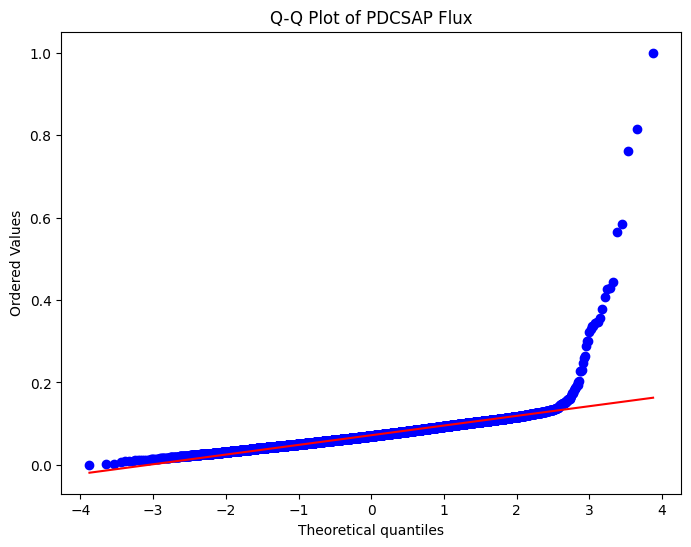
\includegraphics[width=7.5cm,height=5cm]{qqplot.png}
    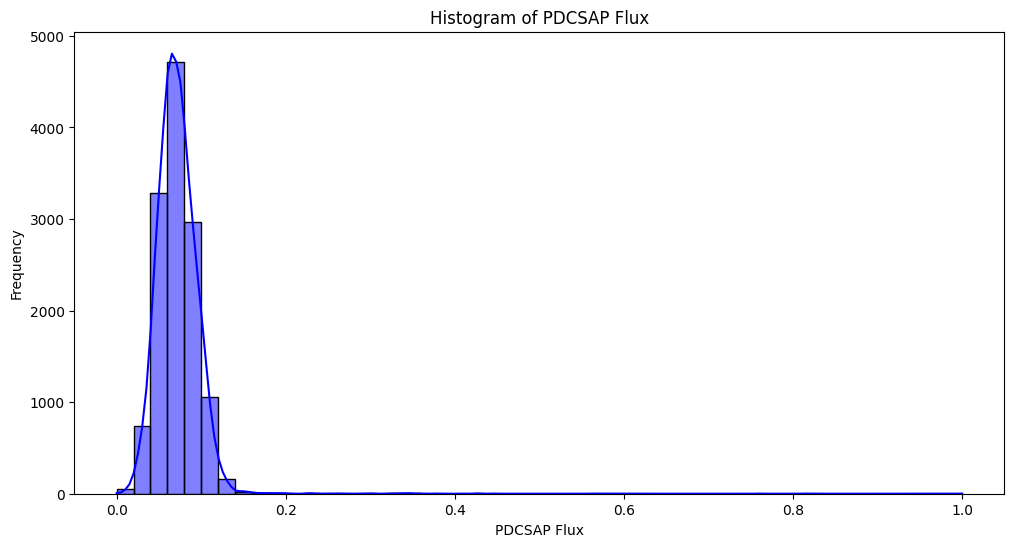
\includegraphics[width=7.5cm,height=5cm]{histogram.png}
    \caption{Graphical Tests for Normality}
\end{figure}

In addition, we conducted two statistical tests (i.e., Anderson-Darling Test and Jarque-Bera Test) used specifically for datasets with more than 5,000 observations. We observed a p-value less than the $5\%$ significance level, indicating that the data is not Normal. Finally, the numeric columns are normalized using MinMaxScaler. The MinMaxScalar was chosen in preference to StandardScalar, as StandardScalar is only used for Gaussian data. The MinMaxScalar scales the values between 0 and 1, ensuring that all features contribute equally to the analysis. This step is beneficial, as it improves the convergence speed and stability of statistical and machine learning algorithms.

\section{Methodology}
Since the dataset is unlabeled, we rely on unsupervised learning methods in order to identify stellar flare events in TESS light curves. In particular, we will be using Density Based Spatial Clustering as well as Outlier Detection using Interquantile Range (IQR). In addition, we will use time series analysis methods of smoothing and differencing (Pietras et al., 2022) to remove noise and detrend the data. 

\subsection{Density Based Spatial Clustering}
With the goal of identifying potential solar flares, we apply a density-based clustering approach, namely using the DBSCAN (Density-Based Spatial Clustering of Application with Noise). Given the noisy nature of the astronomical data, DBSCAN is efficient as it can identify clusters of arbitrary shapes and treat outliers as noise points. DBSCAN has two parameters, Epsilon ($\epsilon$) which is the maximum distance between two samples (neighbors), and min\_samples which corresponds to the minimum amount of points needed to form a dense region. Points within $\epsilon$ distance from a core point are assigned to the same cluster, while points that do not satisfy density requirements are considered noise. For this reason, DBSCAN is favorable for light curve data, where flare events appear as localized, high density bursts of intensity. To tune this model, we use a range of $\epsilon$ and min\_sample values which maximized the separation of flare events from background noise.

\subsection{Outlier Detection using Interquantile Range (IQR)}
We utilize the Interquartile Range (IQR) method for outlier detection and removal. This works by calculating the first quartile (Q1) and third quartile (Q3) of the light curve intensity values and eliminating data points that lie outside the range $[Q1-k \times IQR, Q3+k \times IQR]$. By removing extreme outliers, the overall noise in the data was reduced, improving ability to detect true flare events. Initially, we used a standard value of $k=1.5$ which is typical for detecting mid outliers. However, we later experimented with different values of $k$ to assess the trade off between preserving potential flare events and removing noise.

\subsection{Smoothing}
Smoothing is used to remove noise from the data, which improves model accuracy and pattern detection. We use moving average (MA) smoothing, which averages a fixed number of past values to create a smoothed version of the data.

\subsection{Differencing}
Differencing is used to remove deterministic trends from the data. We apply first-order differencing, where each data point is subtracted from the previous data point. This can be represented as $\nabla x_t= x_t - x_{t-1}$, where $\nabla x_t$ is the differenced value, $x_t$ is the time series value at time $t$, and $x_{t-1}$ is the time series value at time $t-1$.

\section{Results}

\subsection{Flare Detection using DBSCAN}
After post-processing, to identify potential stellar flare events in the TESS mission data, we initially applied DBSCAN using the PDCSAP flux as the clustering feature. The model was fine-tuned using $\epsilon = 0.03$, a small neighborhood size to isolate short-duration spikes, and $min\_samples = 3$, a low threshold to enable detection of smaller clusters. DBSCAN assigns a cluster label to each data point, where noise points (potential flare events) are marked as $-1$. After filtering out low-significance spikes using a flux threshold of 0.1, the model identified 21 flare events.

\begin{figure}[H]
\centering
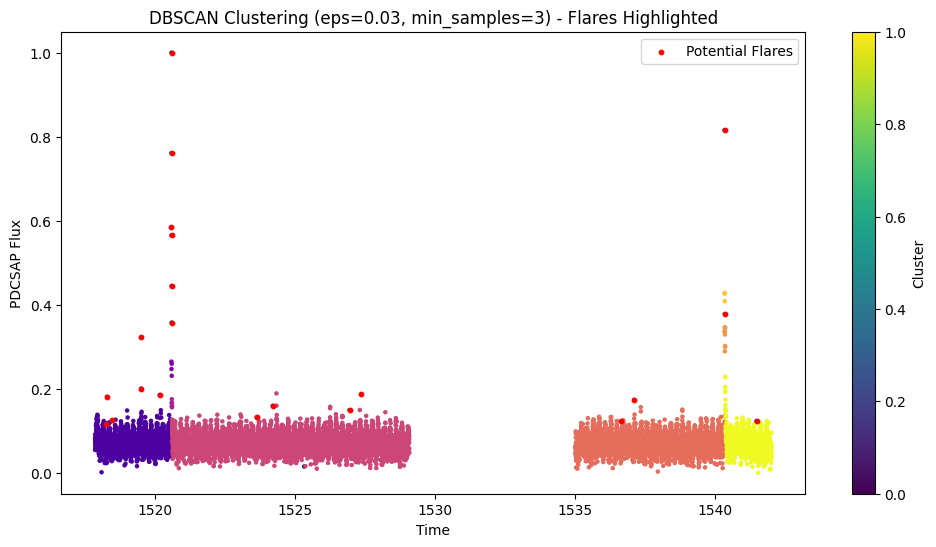
\includegraphics[width=10cm,height=5cm]{dbcan1.png}
\caption{DBSCAN Clustering}
\end{figure}

The results visualized in Figure 2 display a clear separation between flare and non-flare events. The red points representing flare spikes aligned well with high-flux variations. This confirms that DBSCAN efficiently distinguished significant flare events from background noise. However, the relatively low amount of detected flares indicates that more pre-processing could improve sensitivity.

To enhance flare detection, we introduce smoothing; applying an Exponential Moving Average (EMA) with a span of 15 to smooth the data and reduce short-term fluctuations. In addition, we engineered several other features to improve model capability. Some features include:
\begin{itemize}
    \item Flux Gradient: Captures the rate of change in flux
    \item Flux Variance: Measures the local variation in flux values over a rolling window of size 10
    \item Flux Skew: Captures the asymmetry of the flux distribution in a rolling window
    \item Flux Kurtosis: Measures the sharpness of flux peaks
    \item Rolling Count: Tracks the number of significant spikes within a rolling window to identify clustered flare activity.
\end{itemize}
A refined DBSCAN model was applied with parameters $\epsilon = 0.5$ (increased neighborhood size to capture more clusters) and min\_samples = 3. Also, to further filter false positives, we applied a more strict Z-score threshold. These changes lead to an increase in the number of detected flares from 21 to 34, confirming that the additional features improved model sensitivity while reducing noise. The detected flares were more closely aligned with high-flux spikes, suggesting improved model specificity.

\begin{figure}[H]
\centering
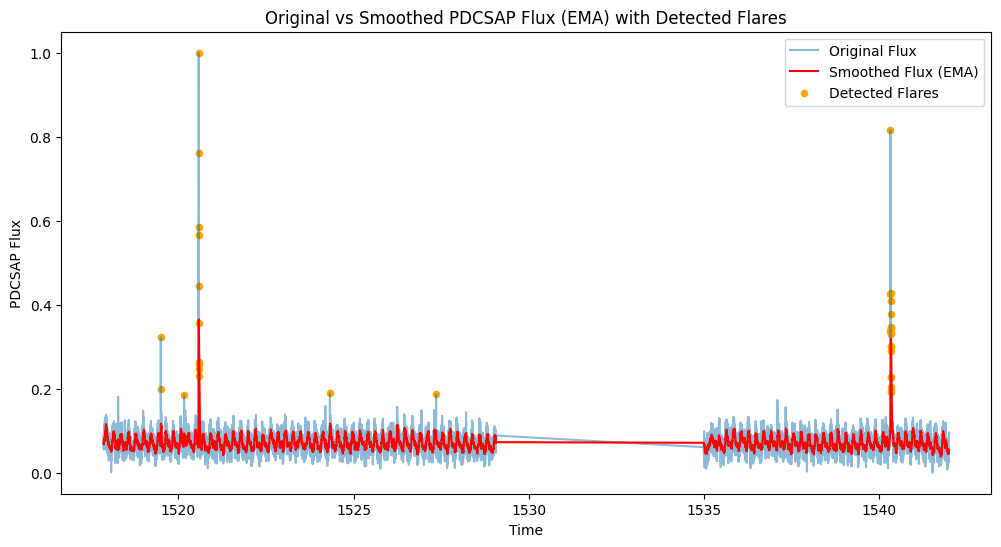
\includegraphics[width=10cm,height=5cm]{dbscan2.png}
\caption{Original vs Smoothed PDCSAP Flux DBSCAN Clustering}
\end{figure}

We evaluated the performance of our DBSCAN models using three distinct metrics for unsupervised learning: Silhouette Score, Davies-Bouldin Index, and Calinski-Harabasz Index. The Silhouette Score measures how well each point fits within its assigned cluster, with values close to +1 indicating good separation and cohesion; negative values implying that many points may be misclassified. The Davies-Bouldin Index evaluates cluster compactness and separation, where lower values are better; a score above 10 generally indicates overlapping or diffuse clusters. The Calinski-Harabasz Index reflects the ratio of between-cluster to within-cluster variance, with higher values suggesting better-defined clusters.

The first DBSCAN model (Figure 2), evaluated with standard clustering metrics, achieved a Silhouette Score of -0.8183, a Davies-Bouldin Index of 18.7451, and a Calinski-Harabasz Index of 5.2391. These metrics indicate very poor model performance, suggesting that the clusters were poorly separated and internally inconsistent. 

On the other hand, the refined DBSCAN model (Figure 3) achieved a Silhouette Score of 0.289, a Davies-Bouldin Index of 0.803, and a Calinski-Harabasz Index of 135.24, indicating marked improvement with reasonably well-separated and compact clusters. While these metrics are still not ideal, they represent a substantial improvement over the first model. Further feature refinement and parameter tuning may enhance the clustering structure, supporting the validity of unsupervised flare grouping in high-dimensional feature space.

\subsection{Outlier Detection and Signal Refinement}
To explore alternative methods for flare detection, I applied the IQR method to identify and remove outliers.

\begin{figure}[H]
\centering
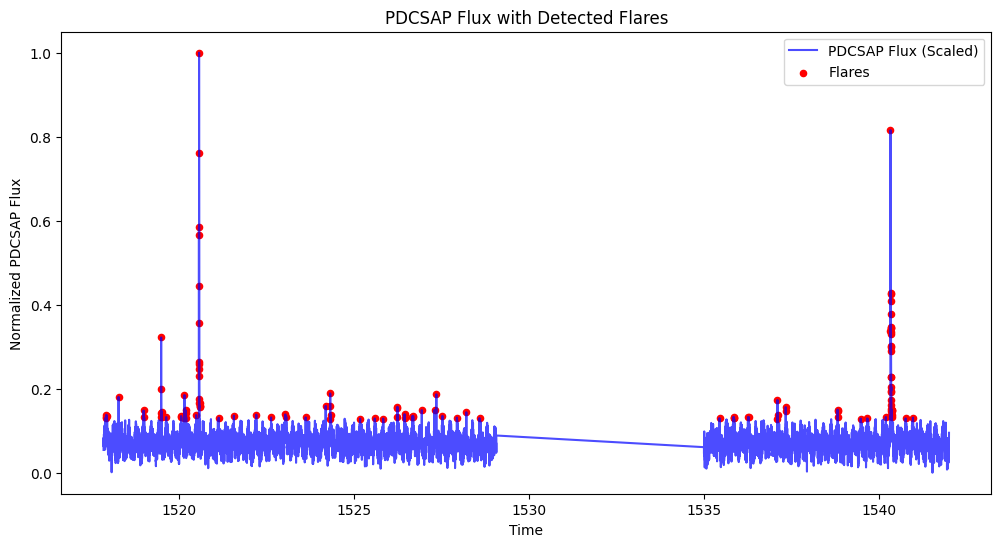
\includegraphics[width=10cm,height=5cm]{iqr.png}
\caption{Outlier Detection using IQR ($k=1.5$)}
\end{figure}

As seen in Figure 4, we initially used $k=1.5$, which detected 116 flares (mu h higher than DBSCAN), which indicated that IQR was overly sensitive and prone to detecting noise as flares. We found that there was a strong autocorrelation signal, so we applied differencing to remove long-term trends and high-frequency variations. This method reduced the number of detected flares from 116 to 64, suggesting that many of the previously detected flares were likely background noise or artifacts of long-term trends. To further stabilize the signal, we used the smoothing method via a rolling mean with a window size of 10.

\begin{figure}[H]
\centering
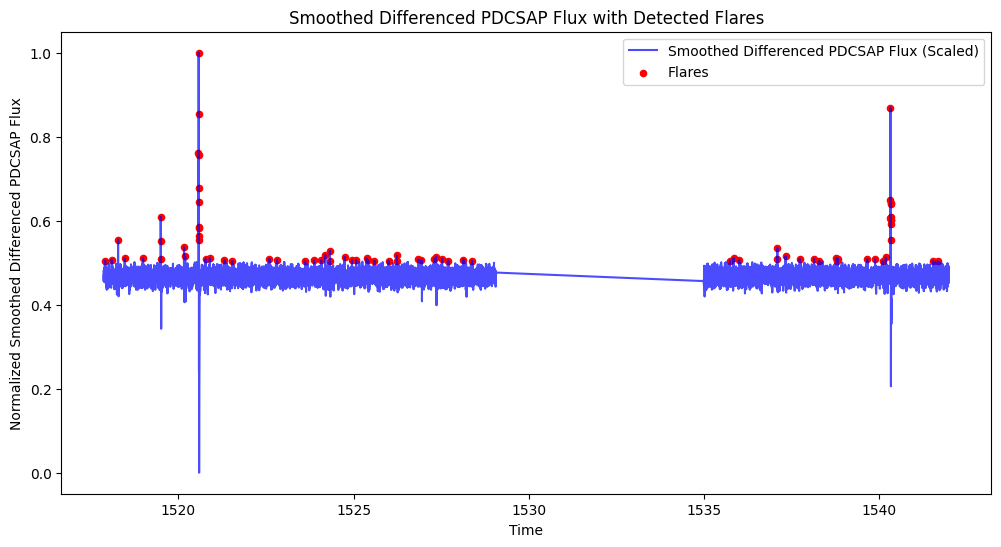
\includegraphics[width=10cm,height=5cm]{iqr+smoothing+differencing.png}
\caption{Smoothed and Differenced Outlier Detection using IQR ($k=1.5$}
\end{figure}

As visualized in Figure 5, smoothing helped reduce noise while preserving genuine flare spikes. Overall, adding smoothing and differencing increased the number of detected flares from 64 to 78 resulting in a cleaner signal and improved sensitivity. Moreover, we tested the impact of varying the IQR multiplier ($k$) to hyper-tune the trade-off between sensitivity and specificity. Increasing k from 1.5 to 2.0 reduced the number of detected flares from 78 to 34, filtering out minor spikes while preserving more significant flare events. It seems a larger multiplier increased specificity but reduced sensitivity to smaller flares, while a lower multiplier increased sensitivity, possibly allowing more false positives. 

\begin{figure}[H]
\centering
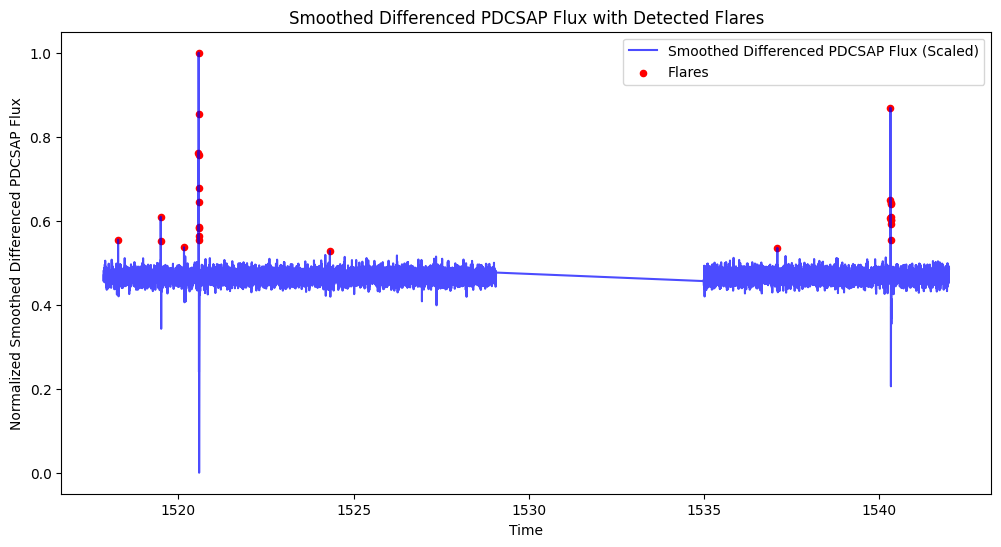
\includegraphics[width=10cm, height=5cm]{kk.png}
\caption{Smoothed and Differenced Outlier Detection using IQR ($k=2$}
\end{figure}

We found that $k=2$ provided the best balance between sensitivity and specificity, as detected flares closely aligned with high-flux events, capturing 26 potential stellar flares, as seen in Figure 6 above. The combination of methods (IQR, differencing, and smoothing) leads to more effective model performance, essentially capturing meaningful flare events while minimizing false positives and background noise.

To evaluate the performance of the IQR flare detection method in the final model (Figure 6), we used a combination of statistical and temporal metrics suited for unsupervised anomaly detection. The outlier ratio measured the proportion of data points flagged as flares relative to the total dataset, with a very low value of 0.20\% indicating high precision and minimal over-flagging of noise. Additionally, we computed the number of distinct flare events, defined as adjacent sequences of flare points, resulting in 7 events over a 24.14-day observation window. The average flare duration, calculated as the number of consecutive flagged points per event, was 3.71 data points, which translates to approximately 7.4 minutes at TESS’s 2-minute cadence \emdash a timescale consistent with short, impulsive stellar flares. These metrics collectively validate the method’s ability to isolate short-duration, high-amplitude anomalies consistent with astrophysical flare signatures, while avoiding false positives from stochastic variability or instrumental noise.

\section{Conclusion}
In conclusion, we successfully explored the detection of stellar flares using data from the Transiting Exoplanet Survey Satellite (TESS). Our primary objective was to develop a robust model for flare detection, leveraging unsupervised learning techniques to differentiate flare events from other forms of stellar activity.

Through a comprehensive analysis of the TESS dataset, we implemented a density-based clustering approach using DBSCAN, which allowed us to identify significant flare events amid the noise in the data. The initial model demonstrated the challenges of detecting flares, as evidenced by the low number of events identified. However, by introducing additional features, we improved the model's sensitivity and specificity, ultimately detecting 34 flare events.

Furthemore, we implemented the Interquartile Range (IQR) method for outlier detection, which initially flagged an excessive number of potential flares. By applying techniques such as differencing and smoothing, we refined our results to isolate genuine flare events more effectively. The final IQR model successfully identified 26 significant flares, providing a clearer understanding of the stellar activity captured in the TESS data.

Overall, this work not only enhances our understanding of stellar flares, but also contributes valuable tools for astronomers studying stellar magnetic activity and its implications for exoplanet habitability. Future research should focus on further refining detection techniques, exploring advanced methods such as machine learning algorithms or Hidden Markov Models (Esquivel, J. A. et al., 2025), and expanding the analysis to other stars within the TESS dataset. This ongoing work aims to provide deeper insight into the intricate processes governing stellar behavior and their potential effects on planetary systems.

\section{References}
\begin{hangparas}{.25in}{1}
Esquivel, J. A., Shen, Y., Leos-Barajas, V., Eadie, G., Speagle, J. S., Craiu, R. V., Medina, A., \& Davenport, J. R. (2025). Detecting stellar flares in photometric data using hidden Markov models. The Astrophysical Journal, 979(2), 141.

Kowalski, A. F. (2024). Stellar flares. Living Reviews in Solar Physics, 21(1).

Pietras, M., Falewicz, R., Siarkowski, M., Bicz, K., \& Preś, P. (2022). Statistical analysis of stellar flares from the first three years of Tess Observations. The Astrophysical Journal, 935(2), 143.

Segura, A. (2018). Star-Planet Interactions and habitability: Radiative effects. Handbook of Exoplanets, 2995–3017.
\end{hangparas}


\end{document}
